\documentclass[xcolor={dvipsnames}]{beamer}
\usepackage{color, colortbl}
\usepackage[ngerman,english]{babel}
\usepackage[T1]{fontenc}
\usepackage{CJKutf8} %japanese
\usepackage{lmodern}
\usepackage[compatibility=false]{caption}
\usepackage{subcaption}
\usepackage{tikz}
\usepackage{textgreek}
\usepackage{tabularx}
\usepackage{booktabs}
\usepackage{siunitx}
\usepackage{appendixnumberbeamer}
\usepackage[absolute,overlay]{textpos} %for positioning the logos where I want
\usepackage{xspace,multicol}

\usepackage{animate}
\usepackage{multimedia}

\mode<presentation>
{
  \usetheme{CambridgeUS}     
  \usecolortheme{lily} 
  \definecolor{beamer@violet}{rgb}{0.5,0.3,0.5} % changed this
  \setbeamercolor{structure}{fg=beamer@violet!70!cyan}
  \setbeamercolor{palette primary}{fg=black, bg=gray!30!white!50!cyan!20!}
  \setbeamercolor{palette secondary}{fg=black, bg=gray!30!white!30!cyan!40!}
  \setbeamercolor*{palette tertiary}{bg=gray!20!white!20!cyan!60!}
  
  \setbeamercolor{frametitle}{fg=cyan!60!white!40!,bg=cyan!80!black}
  \setbeamercolor{title}{fg=cyan!80!black}
  \setbeamercolor{normal text}{fg=black,bg=white}
  \setbeamercolor{alerted text}{fg=beamer@violet}
  \setbeamercolor{example text}{fg=beamer@violet!70!cyan}
  
  \usefonttheme{structureitalicserif} 
  \setbeamertemplate{navigation symbols}{}
  \setbeamertemplate{caption}[numbered]
}
\newcommand{\sidlogo}{
  \setlength{\TPHorizModule}{1pt}
  \setlength{\TPVertModule}{1pt}
   % textblock{}{x,y}: pos(x) = rightUpperCorner + (x * \TPHorizModule), pos(y) = leftUpperCorner - (y * \TPVertModule)
  \begin{textblock}{1}(323,12)
   \includegraphics[width=40pt,height=26pt]{figures/SiD.jpeg}
  \end{textblock}
  } 
\newcommand{\ilclogo}{
  \setlength{\TPHorizModule}{1pt}
  \setlength{\TPVertModule}{1pt}
   % textblock{}{x,y}: pos(x) = rightUpperCorner + (x * \TPHorizModule), pos(y) = leftUpperCorner - (y * \TPVertModule)
  \begin{textblock}{1}(323,12)
   \includegraphics[width=40pt,height=26pt]{figures/ILC.jpeg}
  \end{textblock}
} 
\newcommand{\flukalogo}{
  \setlength{\TPHorizModule}{1pt}
  \setlength{\TPVertModule}{1pt}
   % textblock{}{x,y}: pos(x) = rightUpperCorner + (x * \TPHorizModule), pos(y) = leftUpperCorner - (y * \TPVertModule)
  \begin{textblock}{1}(315,12)
   \includegraphics[width=60pt,height=26pt]{figures/fluka_logo.png}
  \end{textblock}
} 
\newcommand{\ejadelogo}{
  \setlength{\TPHorizModule}{1pt}
  \setlength{\TPVertModule}{1pt}
   % textblock{}{x,y}: pos(x) = rightUpperCorner + (x * \TPHorizModule), pos(y) = leftUpperCorner - (y * \TPVertModule)
  \begin{textblock}{1}(323,12)
   \includegraphics[width=40pt,height=26pt]{figures/EJADE.jpeg}
  \end{textblock}
} 
\newcommand{\BDSsymbol}{
  \setlength{\TPHorizModule}{1pt}
  \setlength{\TPVertModule}{1pt}
   % textblock{}{x,y}: pos(x) = rightUpperCorner + (x * \TPHorizModule), pos(y) = leftUpperCorner - (y * \TPVertModule)
  \begin{textblock}{1}(0,39)
   \includegraphics[width=60pt,height=40pt]{figures/Highlight_BDS.png}
  \end{textblock}
} 
\newcommand{\EXTsymbol}{
  \setlength{\TPHorizModule}{1pt}
  \setlength{\TPVertModule}{1pt}
   % textblock{}{x,y}: pos(x) = rightUpperCorner + (x * \TPHorizModule), pos(y) = leftUpperCorner - (y * \TPVertModule)
  \begin{textblock}{1}(0,39)
   \includegraphics[width=60pt,height=40pt]{figures/Highlight_EXT.png}
  \end{textblock}
} 
\newcommand{\ATFlogo}{
  \setlength{\TPHorizModule}{1pt}
  \setlength{\TPVertModule}{1pt}
   % textblock{}{x,y}: pos(x) = rightUpperCorner + (x * \TPHorizModule), pos(y) = leftUpperCorner - (y * \TPVertModule)
  \begin{textblock}{1}(323,12)
   \includegraphics[width=40pt,height=26pt]{figures/ATF_logo.jpg}
  \end{textblock}
} 
\newcommand{\rhullogo}{
  \setlength{\TPHorizModule}{1pt}
  \setlength{\TPVertModule}{1pt}
   % textblock{}{x,y}: pos(x) = rightUpperCorner + (x * \TPHorizModule), pos(y) = leftUpperCorner - (y * \TPVertModule)
  \begin{textblock}{1}(343,12)
   \includegraphics[width=20pt,height=26pt]{figures/rhul_logo.png}
  \end{textblock}
}

\DeclareSIUnit\year{yr}
\newcommand{\eplus}{e$^+$\xspace}
\newcommand{\eminus}{e$^-$\xspace}

\title[ILC \& Background Simulations]{\textbf{\LARGE\alert{My time in Japan\\\normalsize March - April 2016}\\\vspace*{0.2cm} \small The International Linear Collider \\  Background Simulations \& Optimizing the Final Focus Region}}
\author{\textbf{Anne Sch\"utz}}
\institute{\textbf{KIT, DESY}}
\date{\textbf{\today}}

\titlegraphic{\includegraphics[height=1.0cm]{figures/KIT.png}\hspace*{6cm}~%
   \includegraphics[height=1.2cm]{figures/DESY_Logo.png}
}

\begin{document}

{
\usebackgroundtemplate{
 \tikz\node[opacity=0.1]{\includegraphics[width=\paperwidth]{figures/Iwatecomics.jpg}};
 % \tikz\node[opacity=0.2]{\centering\includegraphics[height=\paperheight]{figures/Iwatecomics.jpg}};
 }
\begin{frame}
  \titlepage
\end{frame}
}

\begin{frame}{Table of contents}
  \tableofcontents
\end{frame}

%--------------------------------------------------------------

\section{Ongoing projects around background simulations}

\begin{frame}{My time in Japan}
\ejadelogo
Thanks to the E-JADE program {\tiny(www.e-jade.eu)} I could go to Japan for two months.\\
\begin{center}
 \includegraphics[width=0.3\textwidth, angle=90]{figures/TokyoUniversity.JPG}
\hspace*{0.3cm}
\includegraphics[width=0.3\textwidth, angle=90]{figures/GreatBuddha.JPG}
\hspace*{0.3cm}
\includegraphics[width=0.3\textwidth, angle=90]{figures/sakura.JPG}\\
\includegraphics[width=0.3\textwidth]{figures/ThreeWiseMonkeys.JPG}
\hspace*{0.1cm}
\includegraphics[width=0.3\textwidth]{figures/Kabukiza.JPG}
\hspace*{0.1cm}
\includegraphics[width=0.3\textwidth]{figures/Kyoto_Fushimi_Inari_shrine.JPG}
\end{center}
\end{frame}

\subsection{Background simulations}

\begin{frame}{Background sources}
\ilclogo
The main sources of background:
\begin{columns}
 \begin{column}{0.55\textwidth}
  \begin{itemize}
    \item Pair background
    \item Bhabha scattering
    \item \textgamma \textgamma $\rightarrow$ hadrons
    \item \emph{Neutrons from the beam dumps}
    \item Background from Final-Focus system (\emph{beam halo collimators}, muon spoilers)
  \end{itemize}
 \end{column}
 \begin{column}{0.45\textwidth}
 \includegraphics[height=0.2\textheight]{figures/beamstrahlung_processes.png}\\
 \includegraphics[height=0.15\textheight]{figures/bhabha_scattering.pdf} 
 \includegraphics[height=0.15\textheight]{figures/gammagamma_hadrons.pdf}
 \end{column}
\end{columns}

\end{frame}




\subsection{Final-Focus system as a background source}
\begin{frame}
\ATFlogo
 \begin{center}
    \LARGE ATF beam operation time - Background study for the beam halo collimator
 \end{center}
\end{frame}

\begin{frame}{Beam Halo collimators}
Vertical collimators suggested for the ILC:\\
 \begin{center}
\includegraphics[width=0.65\textwidth]{figures/ATF2_beamhalo_collimator.pdf}
\end{center}
By driving the collimator blocks into the beam:\\
\begin{itemize}
 \item The beam halo is cut off.
 \item New background is produced.
\end{itemize}

\end{frame}

\begin{frame}{Beam time at ATF2 in March}
\ATFlogo
I joined the ATF2 beam operation time in March.\\
ATF2 is the ILC Final-Focus test bench at KEK in Japan, where the March beam time was dedicated to:
\begin{itemize}
\item Installing a new beam halo collimator
\item Measuring the beam halo
\item Studies of the generated background with a Cherenkov detector
\end{itemize}
\begin{center}
 	\includegraphics[width=0.8\textwidth]{figures/ATF.jpg}
\end{center}
\end{frame}

\begin{frame}{Installed collimator}
\ATFlogo

\begin{center}
\includegraphics[width=\textwidth]{figures/ATF2schematic.pdf}\\
 \includegraphics[width=0.5\textwidth]{figures/Installed_Collimator.jpg}
\end{center}
\end{frame}

\begin{frame}{Data analysis}
\ATFlogo
Data taken with the RHUL Cherenkov detector\\
\vspace*{0.4cm}
 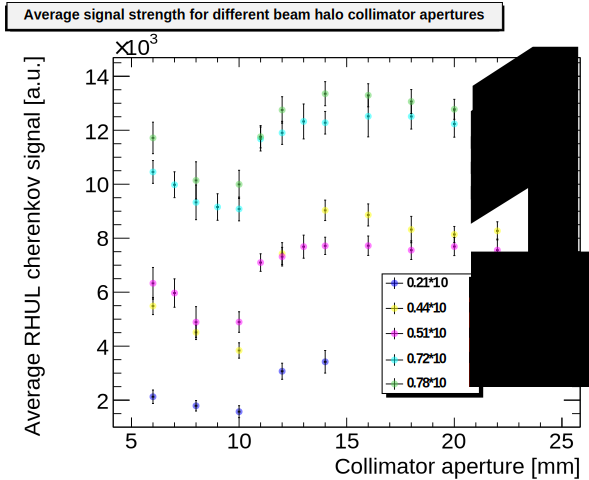
\includegraphics[width=0.55\textwidth]{figures/AverageSignal_perAperture.pdf}
  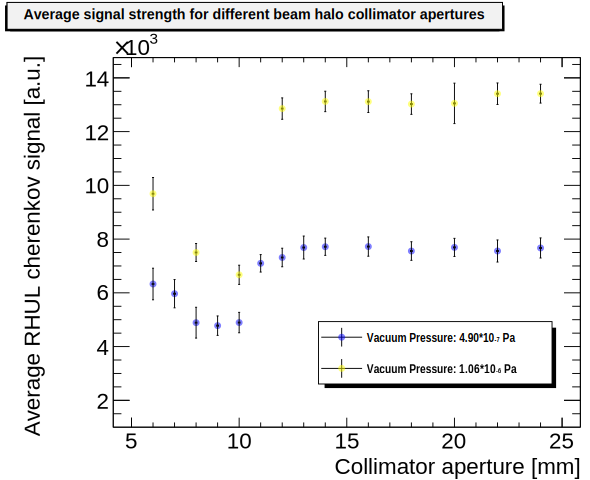
\includegraphics[width=0.55\textwidth]{figures/AverageSignal_perAperture_VacuumPressures.pdf}\\
Background is reduced, but then rises again when collimator jaws are driven closer into the beam halo.\\
\begin{block}{}
The vertical beam size at the location of the collimator was about \SI{0.32}{mm} with an offset of 0.2-\SI{0.5}{mm}.
\end{block}
\end{frame}

\begin{frame}{Data analysis}
\ATFlogo
Data taken with the post-IP background monitor\\
\vspace*{0.3cm}
\begin{center}
  \includegraphics[width=0.8\textwidth]{figures/Nuria_postIP_Bkg_VerticalCollimator.png}\\
\end{center}
Preliminary results by Nuria Fuster Martinez (IFIC, Spain)\\
\Large{$\Rightarrow$ Background is reduced at the IP.}
\end{frame}

\begin{frame}{BDSIM simulation}
\rhullogo
Simulation of ATF2 with BDSIM (developed by RHUL)\\
\begin{itemize}
 \item to compare data taken at ATF with simulation results.
 \item to understand where background particles are generated and stopped exactly.
\end{itemize}

\begin{center}
  \includegraphics[width=0.8\textwidth]{figures/atf_bdsim.png}\\
\end{center}

\begin{columns}
 \begin{column}[c]{0.5\textwidth}
 \centering
\includegraphics[width=0.45\textwidth]{figures/Flange_+z_view2.jpg}\\
\tiny{Beam pipe flange between a rectangular and a circular beam pipe at the location of the Cherenkov detector.}
 \end{column}
 \begin{column}[c]{0.5\textwidth}
I helped Laurie Nevay (RHUL) to improve the ATF2 lattice geometry for BDSIM.
 \end{column}
 \end{columns}
\end{frame}

\subsection{FLUKA simulation of the ILC Beam Dump}
\begin{frame}
 \flukalogo
 \begin{center}
    \LARGE FLUKA simulation of the ILC Beam Dump
 \end{center}
\end{frame}
{
\usebackgroundtemplate{
 \tikz\node[opacity=0.05]{\includegraphics[width=1.1\paperwidth]{figures/TB-0067-300-00-A_stamp.pdf}};
 % \tikz\node[opacity=0.2]{\centering\includegraphics[height=\paperheight]{figures/Iwatecomics.jpg}};
 }
\begin{frame}{FLUKA simulation of the ILC Beam Dump}
\flukalogo
The 16 MW beam is dumped into a water tank after collision.\\Neutrons ($\lesssim$\SI{e10}{\per\square\centi\metre\per\year}) are emitted that radiate the surroundings, and travel back towards the detectors.\\
\vspace*{0.1cm}
%Redoing the simulation studies that were done in 2007, when the design was not decided yet.
Concern about the safety and the functionallity of the beam dump design.
\begin{block}{Simulation step 1}
Simulating the neutrons from the beam dump with FLUKA, using the design drawings by B. Smith~\cite{Smith} to model the dump and the surrounding.
\end{block}

\begin{center}
\includegraphics[height=0.35\textheight]{figures/Front_view_BeamDump_Tomb.png}
\hspace*{0.2cm}
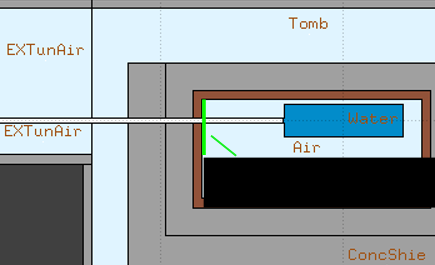
\includegraphics[height=0.35\textheight]{figures/Bird_view_BeamDump_Tomb.png}
\end{center}
\end{frame}

\begin{frame}{FLUKA simulation of the ILC Beam Dump}
\flukalogo
\begin{columns}
\begin{column}[c]{0.4\textwidth}
\includegraphics[height=0.45\textheight]{figures/FLUKA_quadrupole_model.png}\\
\small FLUKA simulation model of one of the ILC EXT lattice quadrupoles.
\end{column}
\begin{column}[c]{0.55\textwidth}
\begin{block}{Simulation step 2}
With Benno List (DESY): Python program to plug the real extraction line lattice into FLUKA.\\
Realistic simulation of the interaction between the neutrons and the lattice.
\end{block}
\begin{block}{Simulation step 3}
Simulating the neutrons reaching the interaction point in a full detector simulation.
\end{block}
\end{column}
\end{columns}
\end{frame}

\begin{frame}{Beam dump simulation goals}
 \flukalogo
 All goals of this study in an overview:
\begin{itemize}
 \item Simulating the neutron flux,
 \item the number of neutrons reaching the IP,
 \item the neutron occupancy in SiD,
 \item the dose of the beam dump surrounding,
 \item the influence of the water composition (amount of deuterium),
 \item the influence of the steel composition of the tank container,
 \item the amount of tritium produced in the water,
 \item the effect of the beam dump design.
\end{itemize}
\vspace*{0.5cm}
\rule{12cm}{.1pt}
\begin{thebibliography}{9}
\setbeamertemplate{bibliography item}[text]
\bibitem{Smith} B. Smith (Rutherford Lab), \emph{Design drawings 0-TB-0067-300-00-A, 0-TB-0067-210-00-A, 0-TB-0067-404-00-A}, Dec. 2006 - Jan. 2007
\end{thebibliography}
\end{frame}
}




\subsection{Bhabha and $\gamma\gamma\rightarrow$hadrons}
\begin{frame}
 \begin{center}
    \LARGE Bhabha and $\gamma\gamma\rightarrow$hadrons
 \end{center}
\end{frame}
\begin{frame}
Available files:
\begin{itemize}
 \item Bhabha (-80\eminus +30\eplus, and +80\eminus -30\eplus):
 \begin{itemize}
  \item sidloi3
 \end{itemize}
 \item $\gamma\gamma\rightarrow$hadrons
  \begin{itemize}
  \item sidloi3
  \item sidloi3 realigned
  \item sidloi3 realigned with anti-did
  \item sidloi3 realigned with circle/wedge cutout
 \end{itemize}
\end{itemize}
\vspace*{0.5cm}
Is there a plan to simulate the bhabha events also for the other SiD geometries?
\end{frame}

\begin{frame}
How to calculate the number of events per train?
\begin{itemize}
 \item Take cross section from the Whizard log files (with which Tim Barklow simulated the events)
 \item Get luminosity per train: Lumi/train=$\frac{Lumi/s}{5}$ (5 trains per second)
\end{itemize}
\begin{columns}[t]
\begin{column}{0.2\textwidth}
\end{column}
\begin{column}[t]{0.5\textwidth}
  \begin{block}{} 
  \#events/train = Lumi/train$ \cdot \sigma$ 
  \end{block}
 \end{column}
 \begin{column}[t]{0.3\textwidth}
\end{column}
\end{columns}
{\color{gray}
Example:
\begin{align*}
 \#events/train &= Lumi/train \cdot \sigma\\
 &= \frac{1.8\cdot10^{34}cm^{-2}s^{-1}}{5} \times 80 nb\\
 &= \sim 2900
\end{align*}
}
Do I need to use a $\gamma\gamma$-luminosity or is that taken care of by the cross sections specified in the Whizard log files?\\
$\rightarrow$ Tim will send a mail on Monday.
\end{frame}

%\section*{The end}
%{
%\usebackgroundtemplate{
% \tikz\node[opacity=0.1]{\includegraphics[width=\paperwidth,resolution=200]{figures/ilc-Comic.png}};
% % \tikz\node[opacity=0.2]{\centering\includegraphics[height=\paperheight]{figures/Iwatecomics.jpg}};
% }
%\begin{frame}
%\ilclogo
%\begin{center}
%\textcolor{RubineRed}{
%	\LARGE Thank you very much for the opportunity\\and the great time!\\
%	\vspace*{0.5cm}
%	\begin{CJK}{UTF8}{min}
%	どうもありがとうございます。
%	\end{CJK}
%}
%\end{center}
%\end{frame}
%}

\end{document}
